\subsection{The First Marker}
The first marker, seen in figure \ref{marker:cross}, contains black crossing lines on a white background.
These are two features which can be used to find the marker so both are tested.

\subsubsection{Using Lines}
The first method is using the black crossing lines by finding all lines in the image.
To do so, all edges must be found.
These are found using a sobel filter and then the number of edges are reduced with the canny edge detector.

The edges are then processed with a Hough transform, writes all possible lines that one edge can produce on top of each other in an image and then returns the lines which have a certain amount of votes.
To limit the scope, the 15 highest voted lines are then selected, so the number of lines are consistent and the threshold for the voting is ignored as it will change from image to image.
The lines are plotted and shown for image 7 in the easy set in figure \ref{fig:lines_in_image}.


\begin{figure}[h]
 \centering
 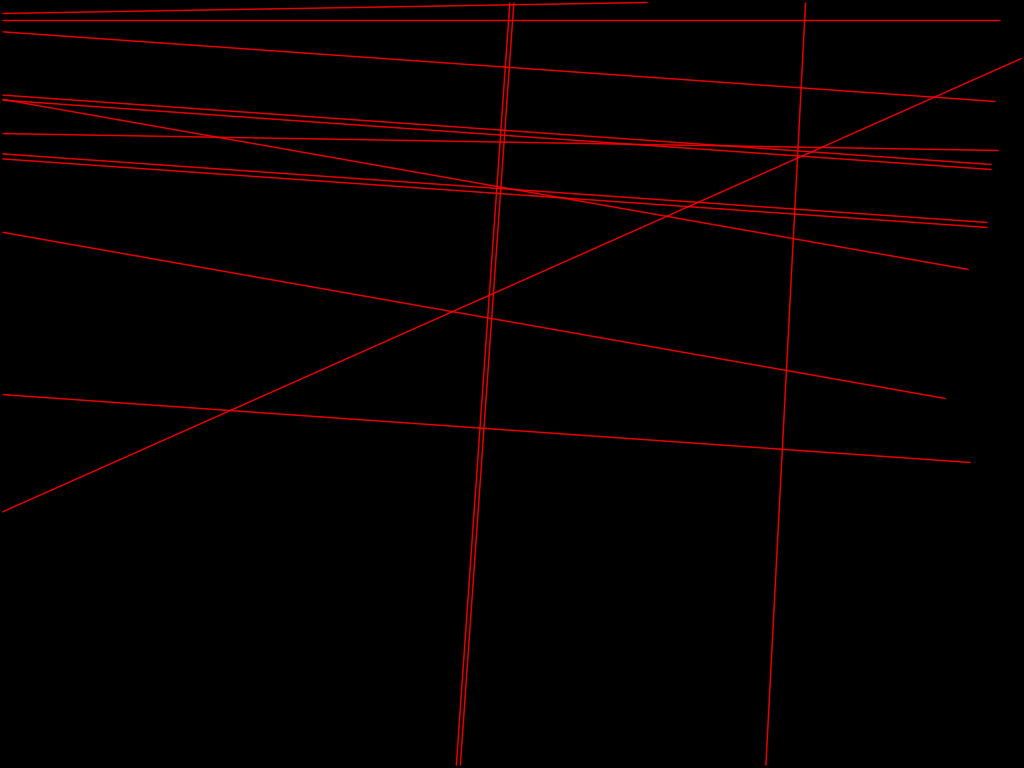
\includegraphics[width=0.6\linewidth]{graphics/Lines_in_image}
 \caption{Lines detected in image 7 from the easy set.}
 \label{fig:lines_in_image}
\end{figure}

The number of lines are then reduced with an analysis.
The lines are given as polar coordinates where a distance to the top left corner of the image and a rotation describes the line that is perpendicular to that point.
The marker contains crossing lines, so lines which have a parallel lines and a 90 degree crossing lines are kept.
Then the crossing point, $C_p$, is calculated in equation \ref{eq:crossing} which was derived appendix \ref{app:crossing_of_two_lines}.

\def\arraystretch{2}
\begin{equation}
% C_p
%  = 
\left[
\begin{array}{c}
 x\\y
\end{array}
\right]
=
% C_p
\left[
\begin{array}{c}
%   \left(
  \frac{ \rho_b - y \cdot  sin(\theta_b) }{ cos(\theta_b) }
%   \right)
  \\
%   \left(
  - \frac{\rho_b - cos(\theta_b) \cdot \frac{\rho_a}{cos(\theta_a)} }{ sin(\theta_a) \cdot \frac{ cos(\theta_b) }{ cos(\theta_a) } + sin(\theta_b) }
%   \right)
  \\
\end{array}
\right]
 \label{eq:crossing}
\end{equation}
\def\arraystretch{\customarrayHeight}

Where $\rho$ is the distance from origin to the line and $\theta$ is the angle from origin. 
In figure \ref{fig:crossing_point} is the crossing point of two lines shown.

\begin{figure}[H]
\centering
\begin{tikzpicture}
 \newcommand{\angleA}{300}
 \newcommand{\radiuA}{1.5}
 \newcommand{\radiuB}{1.5}
 
 \FPeval{\angleB}{\angleA + 90}
 
 \node[name=image] at (0,0) {};
 
 \node[scale=0.3,fill=black, minimum width=15cm, rotate={90 + \angleA}, name=lineA] at ([shift=(\angleA:\radiuA cm)] image.center) {};
 \node[name=midA] at ($(lineA.180)!(image.center)!(lineA.0)$) {};
 \node[above] at (lineA.0) {line$_a$};

 
 \node[scale=0.3,fill=black, minimum width=15cm, rotate={90 + \angleB}, name=lineB] at ([shift=(\angleB:\radiuB cm)] image.center) {};
 \node[name=midB] at ($(lineB.180)!(image.center)!(lineB.0)$) {};
 \node[above] at (lineB.0) {line$_b$};
 
 \FPeval{\rad}{\FPpi/180} %couldn't find the function
 \FPeval{\posX}{round(cos(\angleA * \rad)*\radiuA + cos(\angleB * \rad)*\radiuB,3)}
 \FPeval{\posY}{round(sin(\angleA * \rad)*\radiuA + sin(\angleB * \rad)*\radiuB,3)}
 
 \path (midA); \pgfgetlastxy{\XCoord}{\YCoord};
 \draw[very thick, dashed, green] (image.center) -- (midA.center) node[black, midway, left]       {\(\rho_a\)};
 \draw[very thick, green] (0.5,0) arc(0:{atan(\YCoord/\XCoord)}:0.5cm) node[midway, black, right] {\(\theta_a\)};
 
 \path (midB); \pgfgetlastxy{\XCoord}{\YCoord};
 \draw[very thick, dashed, red] (image.center) -- (midB.center) node[black, midway, above]        {\(\rho_b\)};
 \draw[very thick, red] (0.5,0) arc(0:{atan(\YCoord/\XCoord)}:0.5cm) node[midway, black, right]   {\(\theta_b\)};

 \node[draw, circle,green,very thick]  at (\posX,\posY) {} node[below] at(\posX,\posY) {$C_p$};
\end{tikzpicture}
\caption{Crossing point of two lines.}
\label{fig:crossing_point}
\end{figure}

In figure \ref{fig:crossing_points} is circles within a small area merged and the farthest point in a square is kept.
Testing this, the lines are not always among the highest voted lines, several other lines might be parallel to the marker lines and thus the result gets noisy.
In figure \ref{fig:crossing_points_marker}, it can be seen it working in images where there the lines is detected, but when the all the lines are not detected, 
the algorithm falls apart as it does not have enough points to establish the distance.
This approach worked on 13/30 images in the easy set.
It was not deemed a good solution.

\begin{figure}
 \centering
 \begin{subfigure}{0.49\linewidth}
 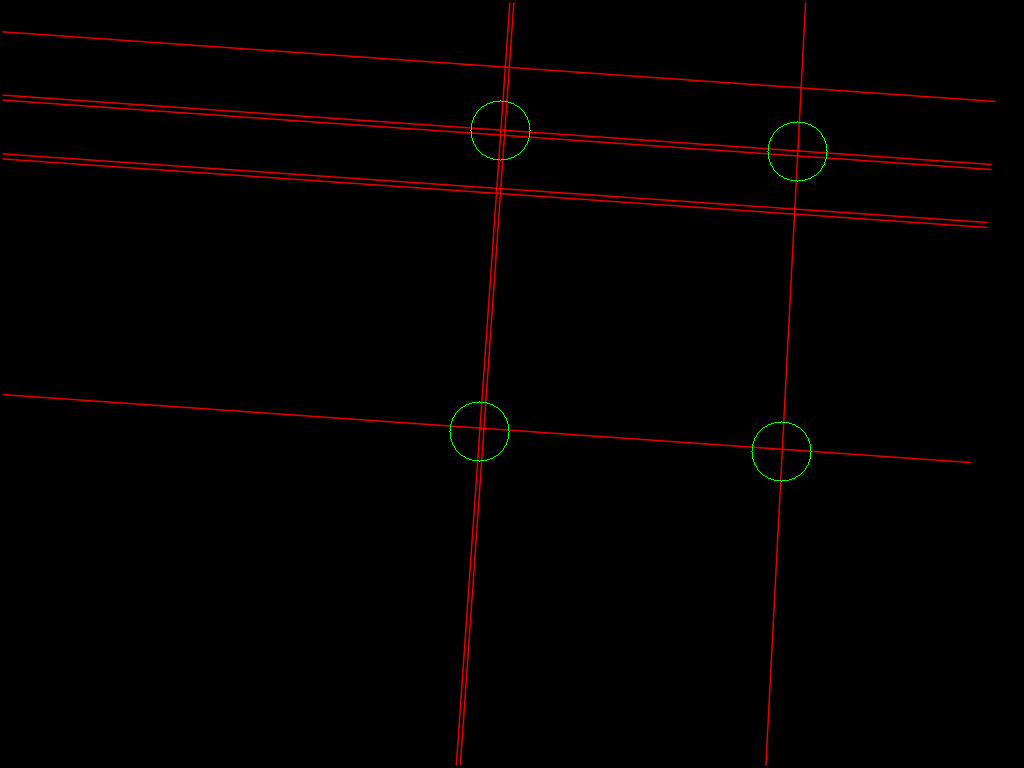
\includegraphics[width=\linewidth]{graphics/Detected_points_marker1a_7}
 \caption{Image 7}
 \label{fig:crossing_points}
 \end{subfigure}
 \begin{subfigure}{0.49\linewidth}
 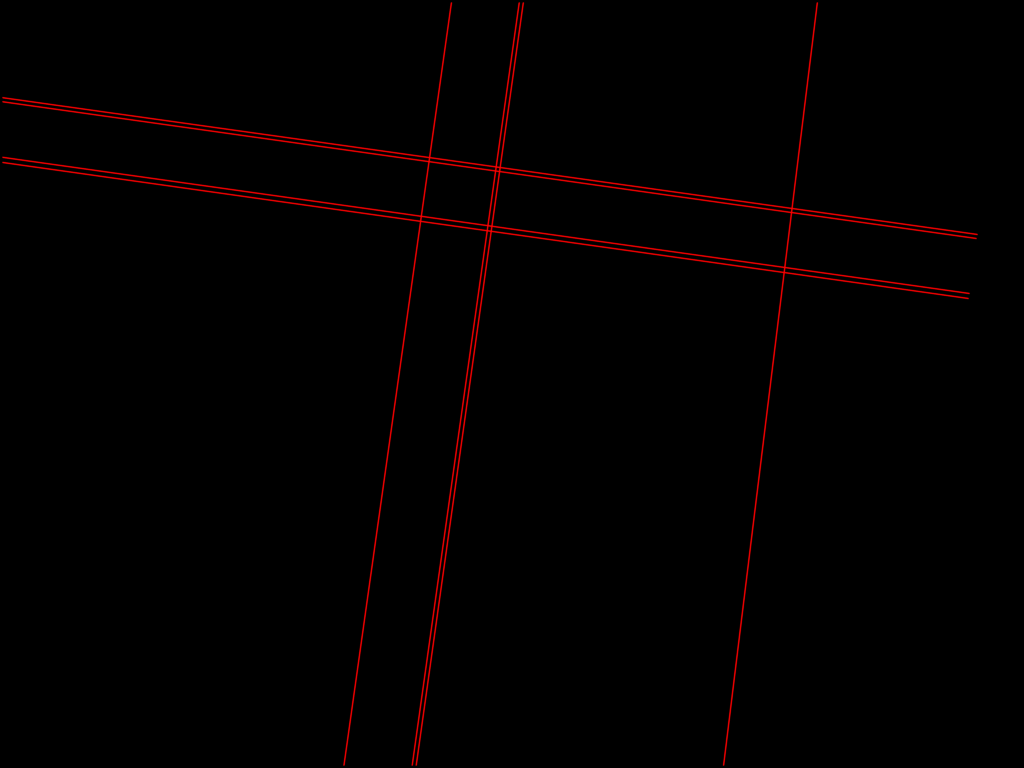
\includegraphics[width=\linewidth]{graphics/Detected_points_marker1a_8}
 \caption{Image 8}
 \end{subfigure}
 \caption{Detected corners of marker 1 from the easy set.}
 \label{fig:crossing_points_marker}
\end{figure}

\subsubsection{Using Contours}
The second method is to use the colors. The marker can be described as a big white plate, separated by the black bars.
If the background contains small white blobs, the marker would be bigger.
If the background is a big white wall, the size of the wall would be larger than the marker so that could be removed based on the size of the object.

The first problem is to select all white in an image.
Converting it to grayscale and selecting high intensity is a way but it does not handle shadows that well and bright areas might be viewed as white.
In figure \ref{fig:threshold_marker1} can the thresholded image be seen and the contours that is detected to be of reasonable size.
The red circle indicates where the marker is found.

\begin{figure}
 \centering
 \begin{subfigure}{0.49\linewidth}
 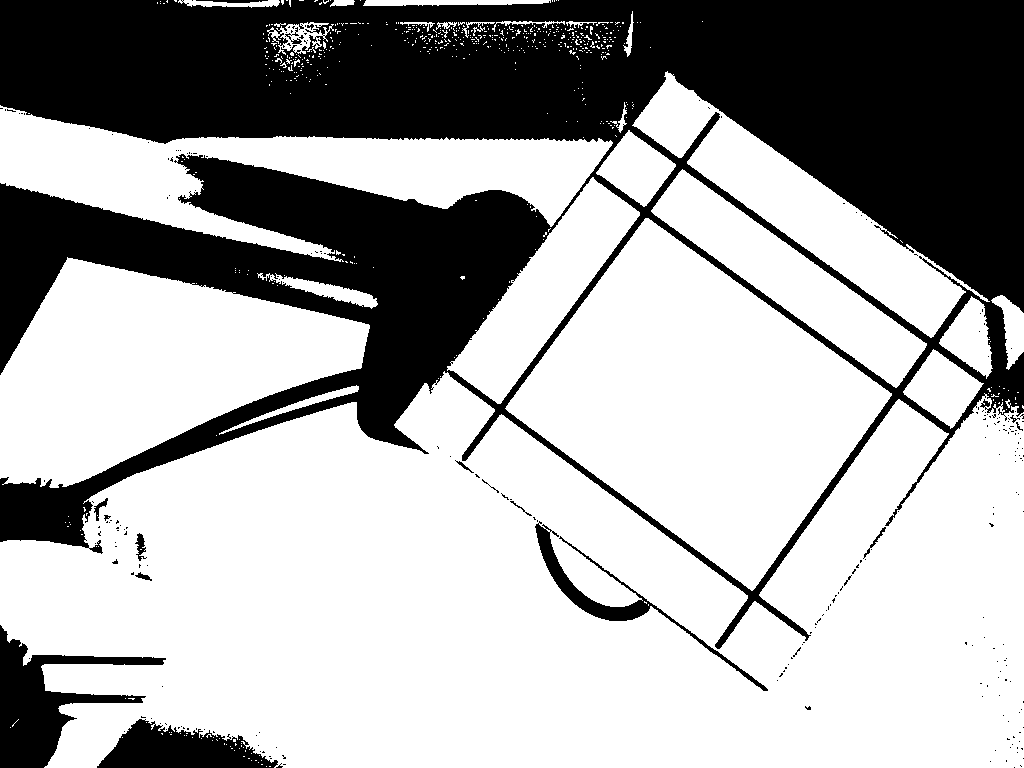
\includegraphics[width=\linewidth]{graphics/threshold_white}
 \caption{White in image.}
 \end{subfigure}
 \begin{subfigure}{0.49\linewidth}
 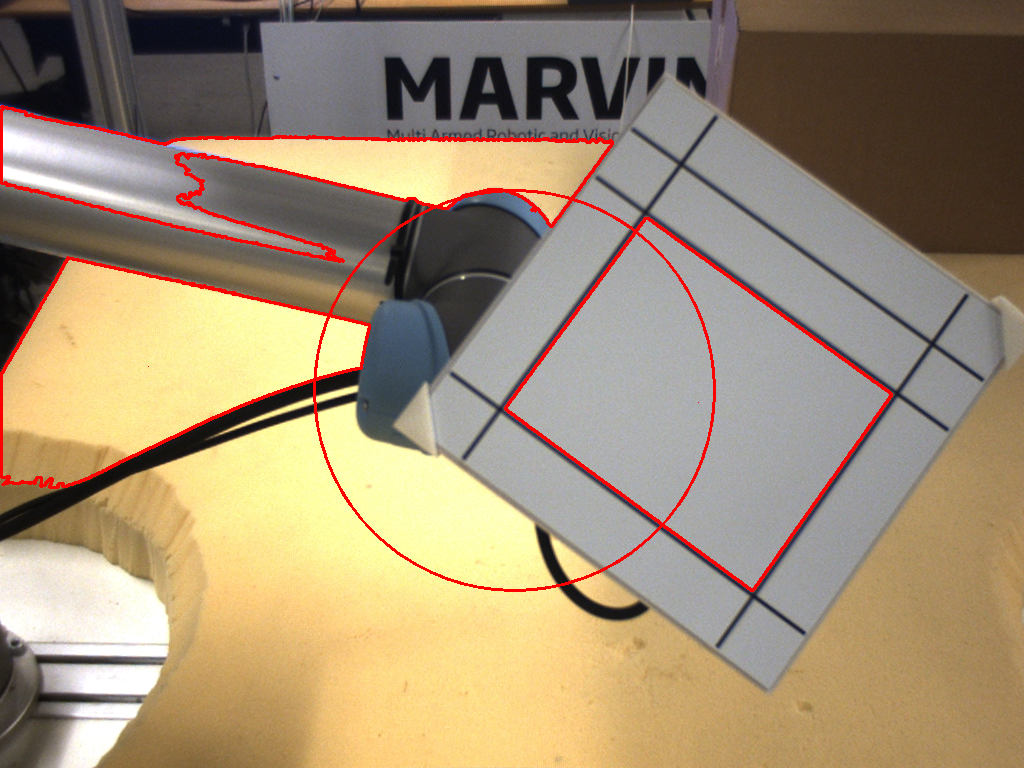
\includegraphics[width=\linewidth]{graphics/threshold_white_contours}
 \caption{Contours detected.}
 \end{subfigure}
 \caption{Detecting the white marker based on grayscale threshold.}
 \label{fig:threshold_marker1}
\end{figure}

A better way to detect the white part is to split the image into Hue Saturation and Value (HSV).
The value is the intensity of the image and selecting the high values gives the same effect as thresholding the grayscale image.
To remove intense colored parts, the saturation must be set. A low saturation would mean the image is not saturated with a color.
0-20\% saturation and 50-100\% intensity was chosen.
In figure \ref{fig:hsv_intensity} is the intensity shown in relation to the HSV values.

\begin{figure}
\centering
 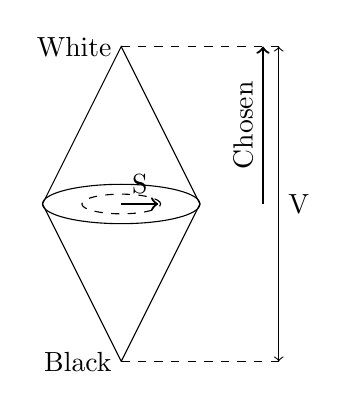
\begin{tikzpicture}
 \draw (0,0) -- (1,2) -- (0,4) -- (-1,2) -- (0,0);
 \draw (0,2) ellipse (1cm and 0.25cm);
 \node[left] at (0,4) {White};
 \node[left] at (0,0) {Black};
 \draw[dashed] (0,2) ellipse (0.5cm and 0.125cm);
 \draw[thick, ->] (0,2) -- ++(0.47,0) node[midway,above,name=s] {S};
 
 \draw[<->] (2,0) -- ++(0,4) node[midway, right] {V};
 \draw[thick, ->] (1.8,2) -- ++(0,2) node[midway, above,rotate=90] {Chosen};
 \draw[dashed] (0,0) -- (2,0) (0,4) -- (2,4);
 \end{tikzpicture}
 \caption[Saturation and intensity in relation to the HSV values.]{Saturation and intensity in relation to the HSV values. Saturation is not to scale in order to illustrate what is taken.}
 \label{fig:hsv_intensity}
\end{figure}


In figure \ref{fig:hsv_marker1} is the white parts and the contours shown for the same area as in figure \ref{fig:threshold_marker1}.
The HSV values are more robust to changes in the environment and is thus better suited for this assignment.

\begin{figure}
 \centering
 \begin{subfigure}{0.49\linewidth}
 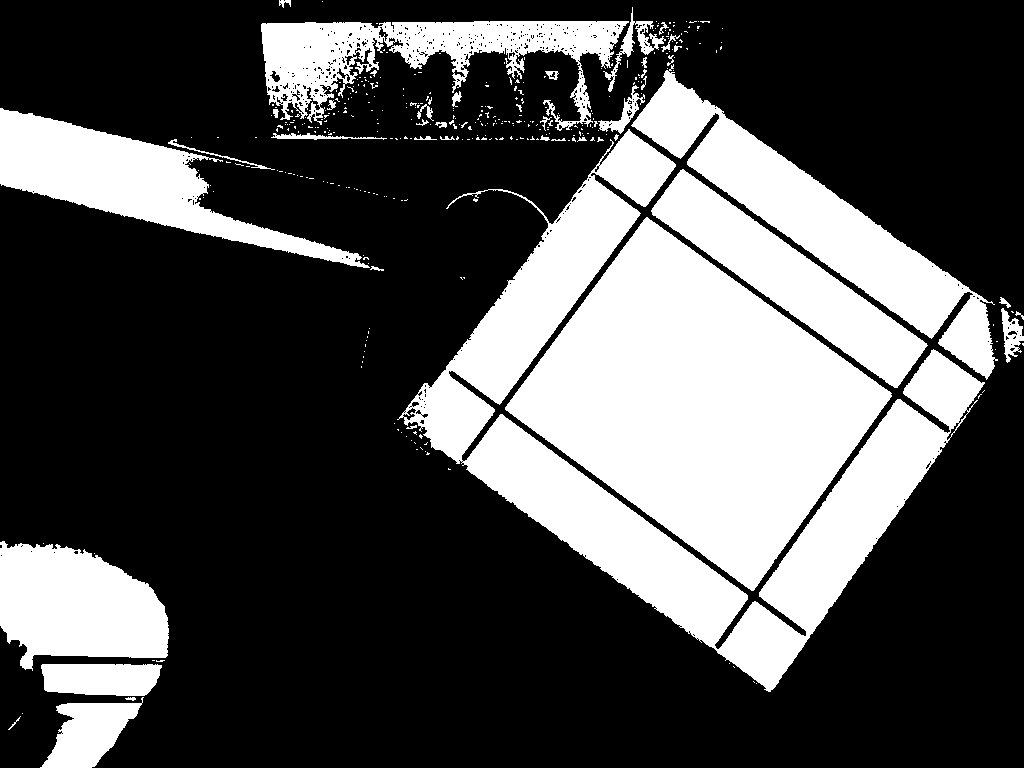
\includegraphics[width=\linewidth]{graphics/hsv_white}
 \caption{White in image.}
 \end{subfigure}
 \begin{subfigure}{0.49\linewidth}
 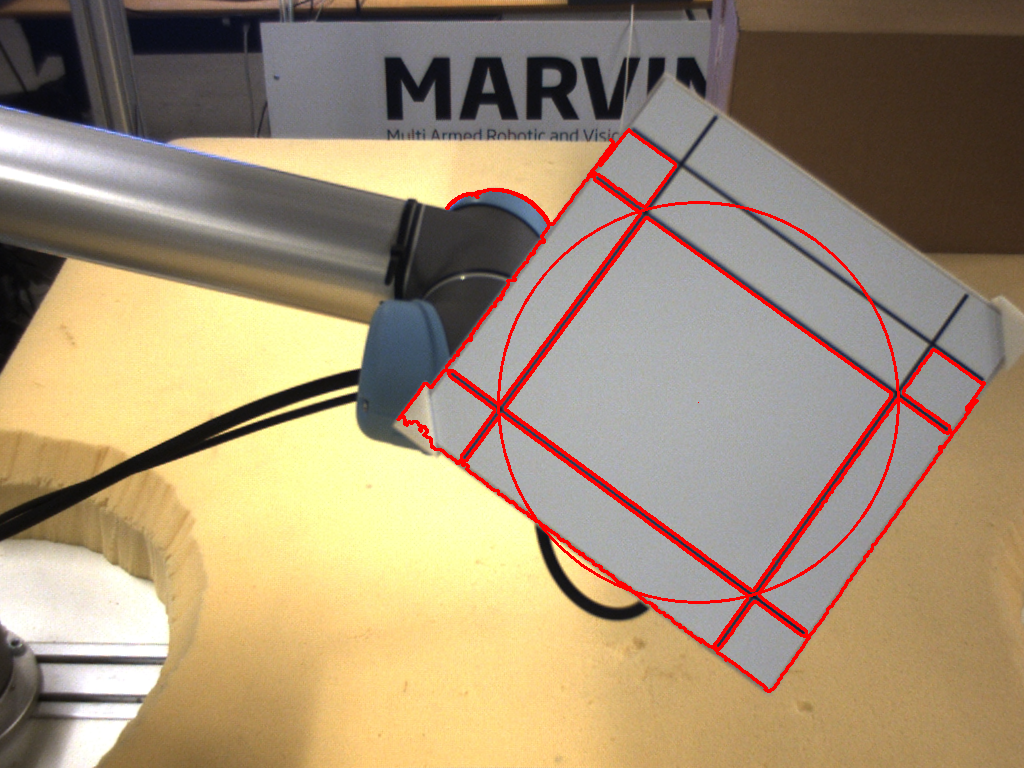
\includegraphics[width=\linewidth]{graphics/hsv_white_contours}
 \caption{Contours detected.}
 \end{subfigure}
 \caption{Detecting the white marker based on HSV threshold.}
 \label{fig:hsv_marker1}
\end{figure}

When the white parts of an image has been detected, the blobs can be found.
By calculating the areas within the contours, the parts within the size of the marker can be found.
Once found, the center of the marker can be found by taking the most compact contour, closest to the center of the image.
As the robot will be following the position of the marker, this is a good estimate, but it also proved to be good in the images used in the test set as the distracting blobs were not placed in the center, behind the marker.
Using this approach the marker can be found on 30/30 images in the easy set and in 52/52 images of the hard set.
\nikolaj{Should I test how many times the marker is found in images where the marker is not there?
I think it might just always detect the marvin sign or something similar.}

